\section{Introduction}
\label{sec:Introduction}
 
This is the template for typesetting LHCb notes and journal papers.
It should be used for any document in LHCb~\cite{LHCb-DP-2008-001} that is to be
publicly available. The format should be used for uploading to
preprint servers and only afterwards should specific typesetting
required for journals or conference proceedings be applied. The main
\latex file contains several options as described in the \latex comment
lines.
 
It is expected that these guidelines are implemented for papers already
before they go into the first collaboration wide review.
These guidelines are here to help proponents write a good paper,
but they also implement the ``LHCb style''. This style is based on
previous decisions by the Editorial Board. They are neither wrong or right,
but help keeping a similar look-and-feel for all LHCb papers.

This template also contains the guidelines for how publications and
conference reports should be written.
The symbols defined in \texttt{lhcb-symbols-def.tex} are compatible with
LHCb guidelines.
 
The front page should be adjusted according to what is
written. Default versions are available for papers, conference reports
and analysis notes. Just comment out what you require in the
\texttt{main.tex} file.
 
This directory contains a file called \texttt{Makefile}.
Typing \texttt{make} will apply all \latex and Bibtex commands
in the correct order to produce a pdf file of the document.
The default \latex compiler is pdflatex, which requires figures
to be in pdf format.
To change to plain \latex, edit line 10 of \texttt{Makefile}.
Typing \texttt{make clean} will remove all temporary files generated by (pdf)latex.
 
There is also a PRL template, which is called \texttt{main-prl.tex}.  You need
to have \textsc{REVTeX 4.1} installed~\cite{REVTeX} to compile this. Typing
\texttt{make prl} produces a PRL-style PDF file. Note that this version is not
meant for LHCb-wide circulation, nor for submission to the arXiv. It is just
available to have a look-and-feel of the final PRL version. Typing \texttt{make
 count} will count the words in the main body.
 
This template now lives on {\tt gitlab} at \url{https://gitlab.cern.ch/lhcb-docs/templates/}. It can be downloaded and used locally, or used to create a new {\tt gitlab} project, or a project on \url{https://www.overleaf.com/}. The latter will be required for paper drafts during EB process.

To ease finding text and comments in  \url{https://www.overleaf.com/} it is recommended to put the main text of the paper in a single file (except for huge documents). Therefore the template is now no longer organised in files by section.

%%%%%%%%%%%%%%%%%%%%%%%%%%%%%%%%%%%%%%%%%%%%%%%%%%%%%%%%%%%%%%%%%%%%%%%%%%%%%%%%%%%%%%%%%%%%%%%%%
\section{General principles}

The main goal is for a paper to be clear. It should be as brief as
possible, without sacrificing clarity. For all public documents,
special consideration should be given to the fact that the reader will
be less familiar with \lhcb than the author.

Here follow a list of general principles that should be adhered to:
\begin{enumerate}

\item Choices that are made concerning layout and typography
  should be consistently applied throughout the document.

\item Standard English should be used (British rather than American)
  for LHCb notes and preprints. Examples: colour, flavour, centre,
  metre, modelled and aluminium. Words ending on -ise or -isation
  (polarise, hadronisation) can be written with -ize or -ization ending but should be consistent.
  The punctuation normally follows the closing quote mark of quoted text, 
  rather than being included before the closing quote.
  Footnotes come after punctuation. 
  Papers to be submitted to an American journal can be written in American
  English instead. Under no circumstance should the two be mixed.

\item Use of jargon should be avoided where possible. ``Systematics'' are ``systematic
  uncertainties'', ``L0'' is ``hardware trigger'', Monte-Carlo'' is ``simulation'', ``penguin'' diagrams
  are best introduced with an expression like ``electroweak loop (penguin) diagrams'', ``cuts'' are ``selection requirements''. The word ``error'' is ambiguous as it can mean the difference between the true and measured values or your estimate thereof. The same applies to event, that we usually take to mean the whole $pp$ collision; candidate or decay can be used instead.''

\item It would be good to avoid using quantities that are internal jargon and/or 
  are impossible to reproduce without the full simulation, \ie\ instead of ``It is 
  required that $\chisqvtx<3$'', to say ``A good quality vertex is required''; 
  instead of ``It is required that $\chisqip>16$'', to say ``The track is 
  inconsistent with originating from a PV''; instead of ``A DLL greater 
  than 20 is required'' say to ``Tracks are required to be identified as kaons''.
  However, experience shows that some journal referees ask for exactly this 
  kind of information, and to safeguard against this, one may consider given 
  some of it in the paper, since even if the exact meaning may be LHCb-specific, 
  it still conveys some qualitative feeling for the significance levels required 
  in the varies steps of the analysis.   
 
\item \latex should be used for typesetting. Line numbering should be
  switched on for drafts that are circulated for comments.

\item The abstract should be concise, and not include citations or
  numbered equations, and should give the key results from the paper.

\item Apart from descriptions of the detector, the trigger and the
  simulation, the text should not be cut-and-pasted from other sources
  that have previously been published.

\item References should usually be made only to publicly accessible
  documents. References to LHCb conference reports and public notes
  should be avoided in journal publications, instead including the
  relevant material in the paper itself.

\item The use of tenses should be consistent. It is recommended to
  mainly stay in the present tense, for the abstract, the description
  of the analysis, \etc; the past tense is then used where necessary,
  for example when describing the data taking conditions.

\item It is recommended to use the passive rather than active voice:
  ``the mass is measured'', rather than ``we measure the mass''.
  Limited use of the active voice is acceptable, in situations where
  re-writing in the passive form would be cumbersome, such as for the
  acknowledgements.  Some leeway is permitted to accommodate different
  author's styles, but ``we'' should not appear excessively in the
  abstract or the first lines of introduction or conclusion.

\item A sentence should not start with a variable, a particle or an acronym.
 A title or caption should not start with an article. 

\item Incorrect punctuation around conjunctive adverbs and the use of 
dangling modifiers are the two most common mistakes of English grammar
in LHCb draft papers. If in doubt, read the wikipedia articles on 
conjunctive adverb and dangling modifier.  

\item When using natural units, at the first occurrence of an energy unit
      that refers to momentum or a radius, add a footnote: ``Natural units
      with $\hbar=c=1$ are used throughout.'' Do this even when somewhere
      a length is reported in units of mm. It's not 100\% consistent, but
      most likely nobody will notice. The problem can be trivially avoided
      when no lengths scales in natural units occur, by omitting the 
      $\hbar$ from the footnote text.

\item Papers dealing with amplitude analyses and/or resonance parameters, 
      other than masses and lifetimes, should use natural units,
      since in these kind of measurements widths are traditionally 
      expressed in MeV and radii in GeV$^{-1}$. It's also the convention
      used by the PDG. 

\item Papers quoting upper limits should give the both the 90\% and
  95\% confidence level values in the text. Only one of these needs to
  be quoted in the abstract and summary.
\end{enumerate}

%%%%%%%%%%%%%%%%%%%%%%%%%%%%%%%%%%%%%%%%%%%%%%%%%%%%%%%%%%%%%%%%%%%%%%%%%%%%%%%%%%%%%%%%%%%%%%%%%
\section{Layout}

\begin{enumerate}

\item Unnecessary blank space should be avoided, between paragraphs or
  around figures and tables.

\item Figure and table captions should be concise and use a somewhat smaller typeface
  than the main text, to help distinguish them. This is achieved by 
  inserting \verb!\small! at the beginning of the caption.
  (NB with the latest version of the file \verb!preamble.tex! this is automatic)
  Figure captions go below the figure, table captions go above the
  table.

\item Captions and footnotes should be punctuated correctly, like
  normal text. The use of too many footnotes should be avoided:
  typically they are used for giving commercial details of companies,
  or standard items like coordinate system definition or the implicit
  inclusion of charge-conjugate processes.\footnote{If placed at the end
    of a sentence, the footnote symbol normally follows the
    punctuation; if placed in the middle of an equation, take care to
    avoid any possible confusion with an index.}$^,$\footnote{The standard footnote reads: ``The inclusion of charge-conjugate processes is implied
    throughout.'' This may need to be modified, for example with ``except in the discussion of asymmetries.''}$^,$\footnote{The LHCb coordinate system is right-handed, with the $z$ axis pointing along the
beam axis, $y$ the vertical direction, and $x$ the horizontal direction. The $(x, z)$ plane is the bending plane
of the dipole magnet.}

\item Tables should be formatted in a simple fashion, without
  excessive use of horizontal and vertical lines.
  Numbers should be vertically aligned on the decimal point and $\pm$ symbol.
  (\verb!\phantom{0}! may help, or defining column separators as \verb!@{\:$\pm$\:}!)
  See Table~\ref{tab:example} for an example. 


\begin{table}[t]
  \caption{
    %\small %captions should be a little bit smaller than main text
    Background-to-signal ratio estimated in a $\pm 50\mevcc$ 
    mass window for the prompt and long-lived background sources, and the 
    minimum bias rate. In this table, as the comparison of numbers among columns
  is not critical, the value $11\pm2$ may also be typeset without the space.}
\begin{center}\begin{tabular}{lr@{\:$\pm$\:}lr@{\:$\pm$\:}ll}
    \hline
    Channel                           & \multicolumn{2}{c}{$B_{\mathrm{pr}}/S$} & \multicolumn{2}{c}{$B_{\mathrm{LL}}/S$}   & MB rate       \\ 
    \hline
    \BsToJPsiPhi              & $ 1.6$ &$0.6$ & $0.51 $ & $ 0.08$ & $\sim 0.3$ Hz \\
    \BdToJPsiKst              & $ 11\phantom{.0}$ & $ 2$ &  $1.5\phantom{0}$ & $ 0.1 $ & $\sim 8.1$ Hz \\
    \decay{\Bp}{\jpsi\Kstarp} & $ 1.6 $ & $ 0.2$ & $0.29 $ & $ 0.06$  & $\sim 1.4$ Hz \\
    \hline
  \end{tabular}\end{center}
\label{tab:example}
\end{table}

\item Figures and tables should normally be placed so that they appear
  on the same page as their first reference, but at the top or bottom
  of the page; if this is not possible, they should come as soon as
  possible afterwards.  They must all be referred to from the text.

\item If one or more equations are referenced, all equations should be numbered using parentheses as shown in
  Eq.~\ref{eq:CKM},
  \begin{equation}
    \label{eq:CKM}
    \Vus\Vubs + 
    \Vcs\Vcbs + 
    \Vts\Vtbs = 0 \ . 
  \end{equation}
  
\item Displayed results like
  \begin{equation*}
    \BF(\decay{\Bs}{\mumu}) < 1.5 \times 10^{-8} \text{ at 95\% CL}
  \end{equation*}
  should in general not be numbered.

\item Numbered equations should be avoided in captions and footnotes.

\item Displayed equations are part of the normal grammar of the
  text. This means that the equation should end in full stop or comma if
  required when reading aloud. The line after the equation should only
  be indented if it starts a new paragraph.

\item Equations in text should be put between a single pair of \$ signs.
  \verb!\mbox{...}! ensures they are not split over several lines.
  So \mbox{$\epsilon_\text{trigger}=(93.9\pm0.2)\%$} is written as
  \verb!\mbox{$\epsilon_\text{trigger}=(93.9\pm0.2)\%$}! and not as
  \verb!$\epsilon_\text{trigger}$=(93.9$\pm$0.2)\%! which generates the oddly-spaced $\epsilon_\text{trigger}$=(93.9$\pm$0.2)\%.

\item Sub-sectioning should not be excessive: sections with more than three
levels of index (1.1.1) should be avoided.

%\item It is generally preferable to itemize a list using numbers rather
%than bullets.

\item Acronyms should be defined the first time they are used,
  \eg ``A dedicated boosted decision tree~(BDT) is designed to select doubly Cabibbo-suppressed~(DCS) decays.''
  The abbreviated words should not be capitalised if it is not naturally
  written with capitals, \eg quantum chromodynamics (QCD),
  impact parameter (IP), boosted decision tree (BDT).
  Avoid acronyms if they are used three times or less.
  A sentence should never start with an acronym and its better to
  avoid it as the last word of a sentence as well.

\end{enumerate}

%%%%%%%%%%%%%%%%%%%%%%%%%%%%%%%%%%%%%%%%%%%%%%%%%%%%%%%%%%%%%%%%%%%%%%%%%%%%%%%%%%%%%%%%%%%%%%%%%
\section{Typography}
\label{sec:typography}

The use of the \latex typesetting symbols defined in the file
\texttt{lhcb-symbols-def.tex} and detailed in the appendices of this
document is strongly encouraged as it will make it much easier to
follow the recommendation set out below.

\begin{enumerate}

\item \lhcb is typeset with a normal (roman) lowercase b.

\item Titles are in bold face, and usually only the first word is
  capitalised.

\item Mathematical symbols and particle names should also be typeset
  in bold when appearing in titles.

\item Units are in roman type, except for constants such as $c$ or $h$
  that are italic: \gev, \gevcc.  The unit should be separated from
  the value with a thin space (``\verb!\,!''),
  and they should not be broken over two lines.
  Correct spacing is automatic when using predefined units inside math mode: \verb!$3.0\gev$! $\to 3.0\gev$.
  Spacing goes wrong when using predefined units outside math mode AND forcing extra space:
  \verb!3.0\,\gev! $\to$ 3.0\,\gev or worse:   \verb!3.0~\gev! $\to$ 3.0~\gev. 

\item  If factors of $c$ are kept, they should be used both for masses and
  momenta, \eg $p=5.2\gevc$ (or $\gev c^{-1}$), $m = 3.1\gevcc$ (or $\gev c^{-2}$). If they are dropped this
  should be done consistently throughout, and a note should be added
  at the first instance to indicate that units are taken with $c=1$.
  Note that there is no consensus on whether decay widths $\Gamma$ are
  in \mev or \mevcc (the former is more common).
  Both are accepted if consistent. 

\item The \% sign should not be separated from the number that precedes it: 5\%, not 5 \%. 
A thin space is also acceptable: 5\,\%, but should be applied consistently throughout the paper.

\item Ranges should be formatted consistently. The recommended form is to use a dash with no spacing around it: 
7--8\gev, obtained as \verb!7--8\gev!. Another possibility is ``7 to 8\gev''.

\item Italic is preferred for particle names (although roman is
  acceptable, if applied consistently throughout).  Particle Data
  Group conventions should generally be followed: \Bd (no need for a
  ``d'' subscript), \decay{\Bs}{\jpsi\phi}, \Bsb,
  (note the long bar, obtained with \verb!\overline!, in contrast to the discouraged short \verb!\bar{B}! resulting in $\bar{B}$), \KS (note the
  uppercase roman type ``S''). 
  This is most easily achieved by using the predefined symbols described in 
  Appendix~\ref{sec:listofsymbols}.

  Italic is also used for particles whose name is an uppercase Greek letter:
  \Upsilonres, \Deltares, \Xires, \Lambdares, \Sigmares, \Omegares, typeset as
  \verb!\Upsilonres!, \verb!\Deltares!, \verb!\Xires!, \verb!\Lambdares!, \verb!\Sigmares!, \verb!\Omegares! (or with the appropriate macros adding charge and subscripts). Paper titles in the bibliography must be adapted accordingly.
  Note that the \Lz baryon has no zero, while the \Lb baryon has one. That's historical.
  
\item Unless there is a good reason not to, the charge of a particle should be
  specified if there is any possible ambiguity 
  ($m(\Kp\Km)$ instead of $m(KK)$, which could refer to neutral kaons).


\item Decay chains can be written in several ways, depending on the complexity and the number of times it occurs. Unless there is a good reason not to, usage of a particular type should be consistent within the paper.
Examples are: 
\decay{\Dsp}{\phi\pip}, with \decay{\phi}{\Kp\Km}; 
\decay{\Dsp}{\phi\pip} (\decay{\phi}{\Kp\Km});  
\decay{\Dsp}{\phi(}{\Kp\Km)\pip}; or
\decay{\Dsp}{[\Kp\Km]_\phi\pip}.

\item Variables are usually italic: $V$ is a voltage (variable), while
  1 V is a volt (unit). Also in combined expressions: $Q$-value, $z$-scale, $R$-parity \etc

\item Subscripts and superscripts are roman type when they refer to a word (such as T
  for transverse) and italic when they refer to a variable (such as
  $t$ for time): \pt, \dms, $t_{\mathrm{rec}}$.

%  This is a test: $f_{\pt}$.

\item Standard function names are in roman type: \eg $\cos$, $\sin$
  and $\exp$.

\item Figure, Section, Equation, Chapter and Reference should be
  abbreviated as Fig., Sect. (or alternatively Sec.), Eq., Chap.\ and
  Ref.\ respectively, when they refer to a particular (numbered) item,
  except when they start a sentence. Table and Appendix are not
  abbreviated.  The plural form of abbreviation keeps the point after
  the s, \eg Figs.~1 and~2. Equations may be referred to either with 
  (``Eq.~(1)'') or without (``Eq.~1'') parentheses, 
  but it should be consistent within the paper.

\item Common abbreviations derived from Latin such as ``for example''
  (\eg), ``in other words'' (\ie), ``and so forth'' (\etc), ``and
  others'' (\etal), ``versus'' (\vs) can be used, with the typography
  shown, but not excessively; other more esoteric abbreviations should be avoided.
  

\item Units, material and particle names are usually lower case if
  spelled out, but often capitalised if abbreviated: amps (A), gauss
  (G), lead (Pb), silicon (Si), kaon (\kaon), but proton (\proton).

%\item The prefix for 1000 (k, \eg kV) should not be confused with
%  that used in computing (K, which strictly speaking denotes $2^{10}$,
%  \eg KB).

\item Counting numbers are usually written in words if they start a
  sentence or if they have a value of ten or below in descriptive
  text (\ie not including figure numbers such as ``Fig.\ 4'', or
  values followed by a unit such as ``4\,cm'').
  The word 'unity' can be useful to express the special meaning of
  the number one in expressions such as: 
``The BDT output takes values between zero and unity''.
% Numbers should not be
%  written as words if they by nature are real numbers that happen to
%  take an integer value, such as $\chisq/\mathrm{ndf} < 4$.

\item Numbers larger than 9999 have a small space between
  the multiples of thousand: \eg 10\,000 or 12\,345\,678.  The decimal
  point is indicated with a point rather than a comma: \eg 3.141.

\item We apply the rounding rules of the
  PDG~\cite{PDG2022}. The basic rule states that if the three
  highest order digits of the uncertainty lie between 100 and 354, we round
  to two significant digits. If they lie between 355 and 949, we round
  to one significant digit. Finally, if they lie between 950 and 999,
  we round up and keep two significant digits. In all cases,
  the central value is given with a precision that matches that of the
  uncertainty. So, for example, the result $0.827 \pm 0.119$ should be
  written as $0.83\pm 0.12$, $0.827\pm 0.367$ should turn into
  $0.8\pm 0.4$, and $14.674\pm0.964$ becomes $14.7\pm1.0$.
  When writing numbers with uncertainty components from
  different sources, \ie statistical and systematic uncertainties, the rule
  applies to the uncertainty with the best precision, so $0.827\pm
  0.367\stat\pm 0.179\syst$ goes to $0.83\pm 0.37\stat\pm 0.18\syst$ and
  $8.943\pm 0.123\stat\pm 0.995\syst$ goes to $8.94\pm 0.12\stat\pm
  1.00\syst$.

\item When rounding numbers, it should be avoided to pad with zeroes
  at the end. So $51237 \pm 4561$ should be rounded as $(5.12 \pm 0.46)
  \times 10^4$ rather than $51200 \pm 4600$. Zeroes are accepted for yields.

\item When rounding numbers in a table, some variation of the rounding
  rules above may be required to achieve uniformity.

\item Hyphenation should be used where necessary to avoid ambiguity,
  but not excessively. For example: ``big-toothed fish'' (to indicate
  that big refers to the teeth, not to the fish), but ``big white
  fish''.  A compound modifier often requires hyphenation
  (\CP-violating observables, \bquark-hadron decays, final-state
  radiation, second-order polynomial), even if the same combination in
  an adjective-noun combination does not (direct \CP violation, heavy
  \bquark hadrons, charmless final state).  Adverb-adjective
  combinations are not hyphenated if the adverb ends with 'ly':
  oppositely charged pions, kinematically similar decay.  Words
  beginning with ``all-'', ``cross-'', ``ex-'' and ``self-'' are
  hyphenated \eg\ cross-section and cross-check. ``two-dimensional''
  is hyphenated. Words beginning with small prefixes (like ``anti'',
  ``bi'', ``co'', ``contra'', ``counter'', ``de'', ``extra'', ``infra'',
  ``inter'', ``intra'', ``micro'', ``mid'', ``mis'', ``multi'', ``non'', ``over'',
  ``peri'', ``post'', ``pre'', ``pro'', ``proto'', ``pseudo'', ``re'', ``semi'',
  ``sub'', ``super'', ``supra'', ``trans'', ``tri'', ``ultra'', ``un'', ``under'' and
  ``whole'') are single words and should not be hyphenated
  \eg\ semileptonic, pseudorapidity, pseudoexperiment, multivariate,
  multidimensional, reweighted,\footnote{Note that we write weighted unless it's the second weighting} preselection, nonresonant, nonzero,
  nonparametric, nonrelativistic, antiparticle,
  misreconstructed and misidentified.

\item Minus signs should be in a proper font ($-1$), not just hyphens
  (-1); this applies to figure labels as well as the body of the text.
  In \latex, use math mode (between \verb!$$!'s) or make a dash (``\verb!--!'').
  In ROOT, use \verb!#minus! to get a normal-sized minus sign. 

\item Inverted commas (around a title, for example) should be a
  matching set of left- and right-handed pairs: ``Title''. The use of
  these should be avoided where possible.

\item Single symbols are preferred for variables in equations, \eg\
  \BF\ rather than BF for a branching fraction.

\item Parentheses are not usually required around a value and its
  uncertainty, before the unit, unless there is possible ambiguity: so
  \mbox{$\dms = 20 \pm 2\invps$} does not need parentheses,
  whereas \mbox{$f_d = (40 \pm 4)$\%} or \mbox{$x=(1.7\pm0.3)\times 10^{-6}$} does.
  The unit does not need to be repeated in
  expressions like \mbox{$1.2 < E < 2.4\gev$}.

\item The same number of decimal places should be given for all values
  in any one expression (\eg \mbox{$5.20 < m_B < 5.34\gevcc$}).

\item Apostrophes are best avoided for abbreviations: if the abbreviated term
  is capitalised or otherwise easily identified then the plural can simply add
  an s, otherwise it is best to rephrase: \eg HPDs, pions, rather
  than HPD's, \piz's, $\pion$s.

\item Particle labels, decay descriptors and mathematical functions are not nouns, and need often to be followed by a noun. 
Thus ``background from \decay{\Bd}{\pip\pim} decays'' instead of ``background from \decay{\Bd}{\pip\pim}'',
and ``the width of the Gaussian function'' instead of ``the width of the Gaussian''.

\item In equations with multidimensional integrations or differentiations, the differential terms should be separated by a thin space and the $\rm d$ should be in roman.
Thus $\int f(x,y) {\rm d}x\,{\rm d}y$ instead $\int f(x,y) {\rm d}x{\rm d}y$ and
$\frac{{\rm d}^2\Gamma}{{\rm d}x\,{\rm d}Q^2}$ instead of $\frac{{\rm d}^2\Gamma}{{\rm d}x{\rm d}Q^2}$.
% The d's are allowed in either roman or italic font, but should be consistent throughout the paper.

\item Double-barrelled names are typeset with a hyphen (\verb!-!), as in Gell-Mann, but joined named use an n-dash (\verb!--!), as in Breit--Wigner. 

\item Avoid gendered words. Mother is rarely needed. Daughter can be a decay product or a final-state particle. Bachelor can be replaced by companion.
\end{enumerate}

%%%%%%%%%%%%%%%%%%%%%%%%%%%%%%%%%%%%%%%%%%%%%%%%%%%%%%%%%%%%%%%%%%%%%%%%%%%%%%%%%%%%%%%%%%%%%%%%%
\section{Detector, simulation and analysis}
\label{sec:Detector}
The paragraph below can be used for the detector
description. Modifications may be required in specific papers to fit
within page limits, to enhance particular detector elements or to
introduce acronyms used later in the text. For journals where strict
word counts are applied (for example, PRL), and space is at a premium,
it may be sufficient to write, as a minimum: ``The LHCb detector is a 
single-arm forward spectrometer covering the pseudorapidity range 
$2 < \eta < 5$, 
described in detail in Refs.~\cite{LHCb-DP-2008-001,LHCb-DP-2014-002}''. 
A slightly longer version could specify the most relevant sub-detectors, {\it e.g} 
``The LHCb 
detector~\cite{LHCb-DP-2008-001,LHCb-DP-2014-002} is a
single-arm forward spectrometer covering the pseudorapidity range $2 < \eta < 5$, designed for
the study of particles containing \bquark\ or \cquark\ quarks. The detector elements that are particularly
relevant to this analysis are: a silicon-strip vertex detector surrounding the $pp$ interaction
region that allows \cquark\ and \bquark\ hadrons to be identified from their characteristically long
flight distance; a tracking system that provides a measurement of the momentum, $p$, of charged
particles; and two ring-imaging Cherenkov detectors that are able to discriminate between
different species of charged hadrons.'' 

\begin{verbatim}
In the following paragraph, references to the individual detector 
performance papers are marked with a * and should only be included 
if the analysis relies on numbers or methods described in the specific 
papers. Otherwise, a reference to the overall detector performance 
paper~\cite{LHCb-DP-2014-002} will suffice. Note also that the text 
defines the acronyms for primary vertex, PV, and impact parameter, IP. 
Remove either of those in case it is not used later on.
\end{verbatim}

The \lhcb detector~\cite{LHCb-DP-2008-001,LHCb-DP-2014-002} is a single-arm forward
spectrometer covering the \mbox{pseudorapidity} range $2<\eta <5$,
designed for the study of particles containing \bquark or \cquark
quarks. The detector includes a high-precision tracking system
consisting of a silicon-strip vertex detector surrounding the $pp$
interaction region~\cite{LHCb-DP-2014-001}\verb!*!, a large-area silicon-strip detector located
upstream of a dipole magnet with a bending power of about
$4{\mathrm{\,T\,m}}$, and three stations of silicon-strip detectors and straw
drift tubes~\cite{LHCb-DP-2013-003,LHCb-DP-2017-001}\verb!*!\footnote{Cite Ref.~\cite{LHCb-DP-2013-003} for Run 1 analyses and Ref.~\cite{LHCb-DP-2017-001} if Run 2 data is used.}
placed downstream of the magnet.
The tracking system provides a measurement of the momentum, \ptot, of charged particles with
a relative uncertainty that varies from 0.5\% at low momentum to 1.0\% at 200\gevc.
The minimum distance of a track to a primary $pp$ collision vertex (PV), the impact parameter (IP), 
is measured with a resolution of $(15+29/\pt)\mum$,
where \pt is the component of the momentum transverse to the beam, in\,\gevc.
Different types of charged hadrons are distinguished using information
from two ring-imaging Cherenkov detectors~\cite{LHCb-DP-2012-003}\verb!*!. 
Photons, electrons and hadrons are identified by a calorimeter system consisting of
scintillating-pad and preshower detectors, an electromagnetic
% calorimeter
and a hadronic calorimeter. Muons are identified by a
system composed of alternating layers of iron and multiwire
proportional chambers~\cite{LHCb-DP-2012-002}\verb!*!.
The online event selection is performed by a trigger~\cite{LHCb-DP-2012-004}\verb!*!, 
which consists of a hardware stage, based on information from the calorimeter and muon
systems, followed by a software stage, which applies a full event
reconstruction.

A more detailed description of the 'full event reconstruction' could be:
\begin{itemize}
\item The trigger~\cite{LHCb-DP-2012-004}\verb!*! consists of a
hardware stage, based on information from the calorimeter and muon
systems, followed by a software stage, in which all charged particles
with $\pt>500\,(300)\mev$ are reconstructed for 2011\,(2012) data.
For triggers that require neutral particles, 
energy deposits in the electromagnetic calorimeter are 
analysed to reconstruct \piz and $\gamma$ candidates.
\end{itemize}

The trigger description has to be specific for the analysis in
question. In general, you should not attempt to describe the full
trigger system. Below are a few variations that inspiration can be
taken from. First from a hadronic analysis, and second from an
analysis with muons in the final state. In case you have to look 
up specifics of a certain trigger, a detailed description of the trigger 
conditions for Run 1 is available in Ref.~\cite{LHCb-PUB-2014-046}. 
{\bf Never cite this note in a PAPER or CONF-note.} 

\begin{itemize}
\item At the hardware trigger stage, events are required to have a muon with high \pt or a
  hadron, photon or electron with high transverse energy in the calorimeters. For hadrons,
  the transverse energy threshold is 3.5\gev.
  The software trigger requires a two-, three- or four-track
  secondary vertex with a significant displacement from any primary
  $pp$ interaction vertex. At least one charged particle
  must have a transverse momentum $\pt > 1.6\gevc$ and be
  inconsistent with originating from a PV.
  A multivariate algorithm~\cite{BBDT,LHCb-PROC-2015-018}\footnote{Ref.~\cite{LHCb-PROC-2015-018} is oly for Run 2.} is used for
  the identification of secondary vertices consistent with the decay
  of a \bquark hadron.
%\item The software trigger requires a two-, three- or four-track
%  secondary vertex with a large sum of the transverse momentum, \pt, of
%  the tracks and a significant displacement from the primary $pp$
%  interaction vertices~(PVs). At least one track should have $\pt >
%  1.7\gevc$ and \chisqip with respect to any
%  primary interaction greater than 16, where \chisqip is defined as the
%  difference in \chisq of a given PV reconstructed with and
%  without the considered track.\footnote{If this sentence is used to define \chisqip
%  for a composite particle instead of for a single track, replace ``track'' by ``particle'' or ``candidate''}
% A multivariate algorithm~\cite{BBDT} is used for
%  the identification of secondary vertices consistent with the decay
%  of a \bquark hadron.
\item The $\decay{\Bd}{\Kstarz\mumu}$ signal candidates are first required
      to pass the hardware trigger, which selects events containing at least
      one muon with transverse momentum $\pt>1.48\gevc$ in the 7\tev data or
      $\pt>1.76\gevc$ in the 8\tev data.  In the subsequent software
      trigger, at least one of the final-state particles is required to 
      have $\pt>1.7\gevc$ in the 7\tev data or $\pt>1.6\gevc$ in the 8\tev 
      data, unless the particle is identified as a muon in which case 
      $\pt>1.0\gevc$ is required. The final-state particles that 
      satisfy these transverse momentum criteria are also required 
      to have an impact parameter larger than $100\mum$ with respect 
      to all PVs in the event. Finally, the tracks of two or more of 
      the final-state particles are required to form a vertex that is 
      significantly displaced from any PV." 

%  Candidate events are first required to pass the hardware trigger,
%  which selects muons with a transverse momentum $\pt>1.48\gevc$ 
%  in the 7\tev data or $\pt>1.76\gevc$ in the 8\tev data.
%  In the subsequent software trigger, at least
%  one of the final-state particles is required to have both
%  $\pt>0.8\gevc$ and impact parameter larger than $100\mum$ with respect to all
%  of the primary $pp$ interaction vertices~(PVs) in the
%  event. Finally, the tracks of two or more of the final-state
%  particles are required to form a vertex that is significantly
%  displaced from the PVs.
\end{itemize}

For analyses using the Turbo stream, the following paragraph may 
be used to describe the trigger.
\begin{itemize}
\item  The online event selection is performed by a trigger, which consists of a hardware stage followed by a two-level software stage. In between the two software stages, an alignment and calibration of the detector is performed in near real-time and their results are used in the trigger~\cite{LHCb-PROC-2015-011}.
      The same alignment and calibration information is propagated 
      to the offline reconstruction, ensuring consistent and high-quality 
      particle identification (PID) information between the trigger and 
      offline software. The identical performance of the online and offline 
      reconstruction offers the opportunity to perform physics analyses 
      directly using candidates reconstructed in the trigger 
      \cite{LHCb-DP-2012-004,LHCb-DP-2016-001} 
      which the present analysis exploits. The storage of only the triggered
      candidates enables a reduction in the event size by an order 
      of magnitude.
\end{itemize}

An example to describe the use of both TOS and TIS candidates:
\begin{itemize}
\item In the offline selection, trigger signals are associated with reconstructed particles.
%Selection requirements can therefore be made not only on the trigger requirement,
%but on whether the decision was due to the signal candidate, other particles produced in the $pp$ collision, or a combination of both.
Selection requirements can therefore be made on the trigger selection itself
and on whether the decision was due to the signal candidate, other particles produced in the $pp$ collision, or a combination of both.
\end{itemize}

A good example of a description of long and downstream \KS is given in 
Ref.~\cite{LHCb-PAPER-2014-006}:
\begin{itemize}
\item
Decays of \decay{\KS}{\pip\pim} are reconstructed in two different categories:
the first involving \KS mesons that decay early enough for the
pions to be reconstructed in the vertex detector; and the
second containing \KS that decay later such that track segments of the
pions cannot be formed in the vertex detector. These categories are
referred to as \emph{long} and \emph{downstream}, respectively. The
long category has better mass, momentum and vertex resolution than the
downstream category.
\end{itemize}

Before describing the simulation, explain in one sentence why simulation is needed.
The following paragraph can act as inspiration but
with variations according to the level of detail required and if
mentioning of \eg \photos and {\tt ReDecay} is required.
\begin{itemize}
\item Simulation is required to model the effects of the detector acceptance and the
  imposed selection requirements.
  In the simulation, $pp$ collisions are generated using
  \pythia~\cite{Sjostrand:2007gs,*Sjostrand:2006za} 
  (In case only \pythia 6 is used, remove \verb=*Sjostrand:2007gs= from this citation.)
  with a specific \lhcb configuration~\cite{LHCb-PROC-2010-056}.
  Decays of unstable particles
  are described by \evtgen~\cite{Lange:2001uf}, in which final-state
  radiation is generated using \photos~\cite{davidson2015photos}.
  The interaction of the generated particles with the detector, and its response,
  are implemented using the \geant
  toolkit~\cite{Allison:2006ve, *Agostinelli:2002hh} as described in
  Ref.~\cite{LHCb-PROC-2011-006}. 
  %With the exception of the signal decay, the
  %simulated event is reused
  %multiple times
  The underlying $pp$ interaction is reused multiple times, with an independently generated signal decay for each~\cite{LHCb-DP-2018-004}.\footnote{This sentence is to be added only if {\tt ReDecay} is used.}
\end{itemize}

A quantity often used in LHCb analyses is \chisqip. When mentioning it in 
a paper, the following wording could be used: ``$\ldots$\chisqip\ with respect 
to any primary interaction vertex greater than X, where \chisqip\ is defined as 
the difference in the vertex-fit \chisq of a given PV reconstructed with and
without the track under consideration/being considered.''\footnote{If this
sentence is used to define \chisqip\ for a composite particle instead of 
for a single track, replace ``track'' by ``particle'' or ``candidate''.}
This definition can then be used to define the associated PV.\footnote{known as ``best'' PV in \davinci. Use the word ``associated'', not ``best''.} However,
  \chisqip should not be defined just to explain which PV is taken as associated. Instead one can write ``The PV that fits best to the flight direction of the \B candidate is taken as the associated PV.''
  
Many analyses depend on boosted decision trees. It is inappropriate to
use TMVA~\cite{Hocker:2007ht,*TMVA4} as sole reference as that is
merely an implementation of the BDT algorithm.
Rather it is suggested to write: ``In this paper we use a 
boosted decision tree~(BDT)~\cite{Breiman,AdaBoost} implemented in the TMVA
toolkit~\cite{Hocker:2007ht,*TMVA4} to separate signal from background''. 

When describing the integrated luminosity of the data set, do not use
expressions like ``1.0\invfb of data'', but \eg 
``data sample corresponding to an integrated luminosity of 1.0\invfb'', 
or ``a sample of data obtained from 3\invfb of integrated luminosity''. 

For analyses where the periodical reversal of the magnetic field is crucial, 
\eg in measurements of direct \CP violation, the following description can be
used as an example phrase: 
\begin{itemize} \item  The magnetic field deflects oppositely charged particles in opposite
directions and this can lead to detection asymmetries. Periodically
reversing the magnetic field polarity throughout the data-taking almost cancels
the effect. The configuration with the magnetic field pointing upwards (downwards), 
\MagUp (\MagDown), bends positively (negatively) charged particles
in the horizontal plane towards the centre of the LHC ring.\end{itemize}
Only use the \MagUp, \MagDown symbols if they are used extensively in tables or figures.

If the momentum scaling has been applied and is relevant, add text along the lines of
\begin{itemize} \item The momentum scale is calibrated using samples of $\decay{\jpsi}{\mumu}$ 
and $\decay{\Bu}{\jpsi\Kp}$~decays collected concurrently
with the~data sample used for this analysis~\cite{LHCb-PAPER-2012-048,LHCb-PAPER-2013-011}.
The~relative accuracy of this
procedure is estimated to be $3 \times 10^{-4}$ using samples of other
fully reconstructed $\bquark$~hadrons, $\PUpsilon$~and
$\KS$~mesons. \end{itemize}

When describing  "blind analysis", consider adding the following sentence:
\begin{itemize} 
\item In order to avoid experimenter's bias, the results of the analysis were
not examined until the full procedure had been finalised. 
\end{itemize}

% ===============================================================================
% Purpose: including figures in the standard template
% Author: Tomasz Skwarnicki, Ulrik Egede
% Created on: 2010-09-24
% ===============================================================================

%%%%%%%%%%%%%%%%%%%%%%%%%%%%%%%%%%%%%%%%%%%%%%%%%%%%%%%%%%%%%%%%%%%%%%%%%%%%%%%%%%%%%%%%%%%%%%%%%
\section{Figures}
\label{sec:Figures}

A standard \lhcb style file for use in production of figures in \root
is in the \urania package \texttt{RootTools/LHCbStyle} or directly in
\git at
\texttt{https://gitlab.cern.ch/lhcb/Urania/tree/master/RootTools/LHCbStyle}.
It is not mandatory to use this style, but it makes it easier to
follow the recommendations below. For labelling the axis and legends
it is recommended to use (as in the examples) the same text fonts as
in the main text. When using ROOT to produce the plots, use the
upright symbol font for text. The slanted font exists, but does not
look good. It is also possible to use consistently upright sans-serif
fonts for the text (slide style). However, styles should not be
mixed. For particle symbols, try to use the same font (roman/italic)
as is used in the text.

Pull plots are control plots, which are useful in analysis notes.  
Normally they are not shown in papers, unless one wants to emphasise 
regions where a fit does not describe the data. For satisfactory 
fits, in a paper it is sufficient to simply state the fact and/or
give the $\chisq/$ndf.


Figure~\ref{fig:example} shows an example of how to include an eps
or pdf figure with the \texttt{\textbackslash includegraphics} command
(eps figures will not work with \texttt{pdflatex}). Note that if the
graphics sits in \texttt{figs/myfig.pdf}, you can just write
\texttt{\textbackslash includegraphics\{myfig\}} as the \texttt{figs}
subdirectory is searched automatically and the extension \texttt{.pdf}
(\texttt{.eps}) is automatically added for \texttt{pdflatex}
(\texttt{latex}).
%%%%%%%%%%%%%%%%%%%%%%%%%%%%%%%%%%%%%%%%
\begin{figure}[tb]
  \begin{center}
    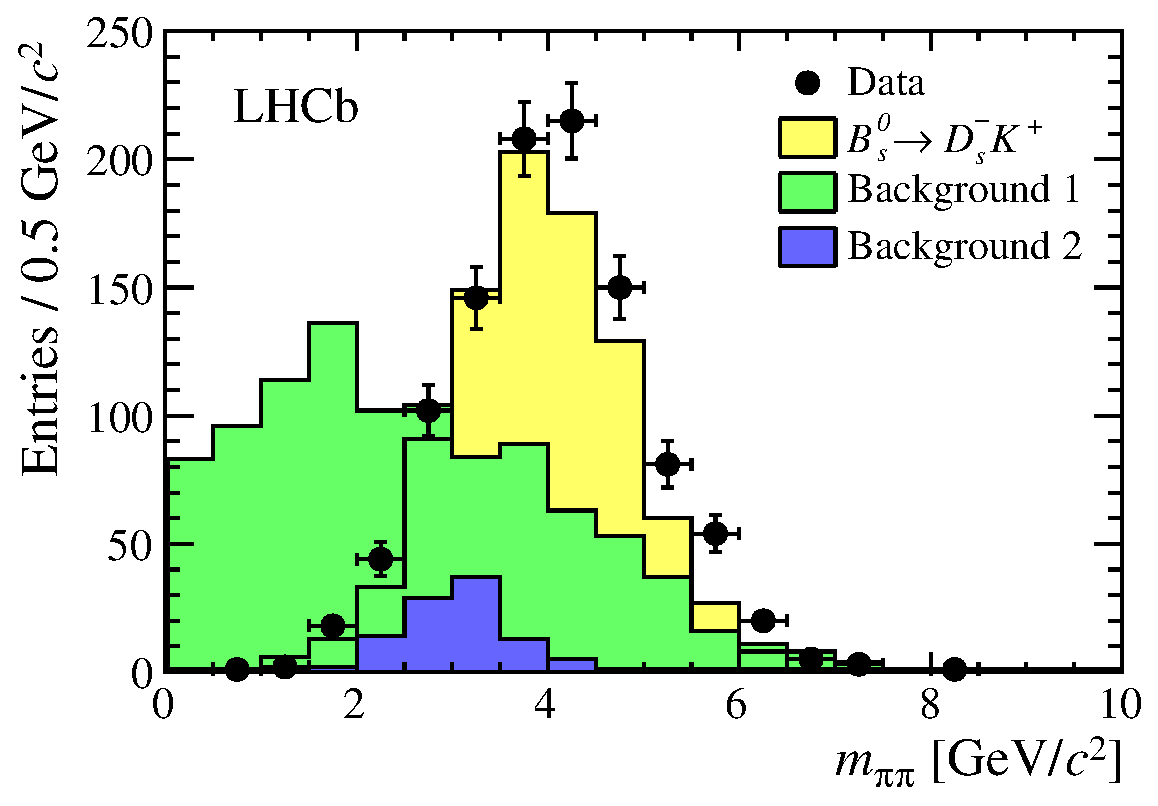
\includegraphics[width=0.49\linewidth]{Example1DPlot-python-1}\put(-32,133){(a)}
    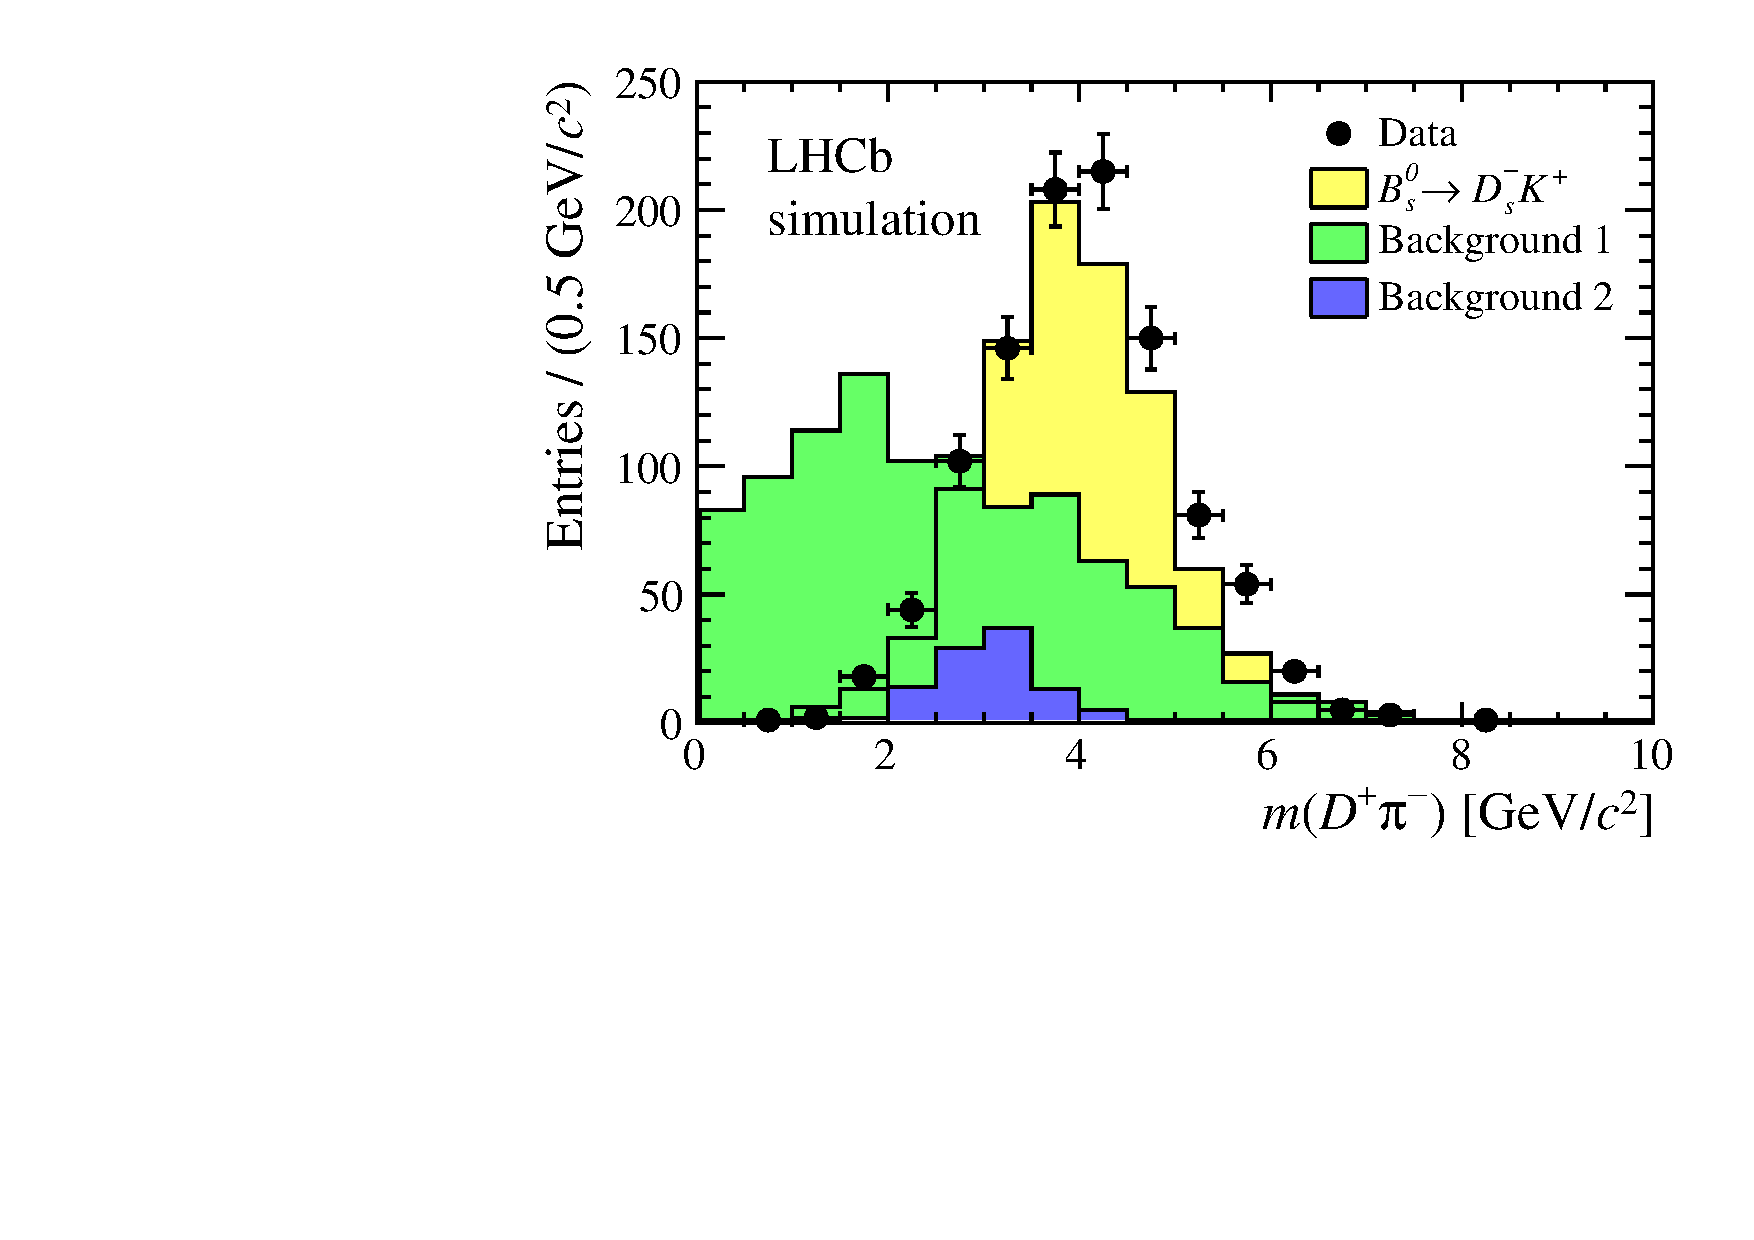
\includegraphics[width=0.49\linewidth]{Example1DPlot-python-1_sim}\put(-32,133){(b)}
    \vspace*{-0.5cm}
  \end{center}
  \caption{
    %\small %captions should be a little bit smaller than main text
    Example plots for (a) data and (b) simulation using the \lhcb style from the \urania package
    \texttt{RootTools/LHCbStyle}. The signal data is shown as points
    with the signal component as yellow (light shaded), background 1 as green
    (medium shaded) and background 2 as blue (dark shaded).}
  \label{fig:example}
\end{figure}
%%%%%%%%%%%%%%%%%%%%%%%%%%%%%%%%%%%%%%%%

\begin{enumerate}
\item Before you make a figure you should ask yourself what message
  you want to get across. You don't make a plot ``because you can''
  but because it is the best illustration of your argument. 
  
\item Figures should be legible at the size they will appear in the
  publication, with suitable line width.  Their axes should be
  labelled, and have suitable units (e.g. avoid a mass plot with
  labels in \mevcc if the region of interest covers a few \gevcc
  and all the numbers then run together).  Spurious background shading
  and boxes around text should be avoided.

\item For the $y$-axis, ``Entries'' or ``Candidates'' is appropriate in case no
background subtraction has been applied. Otherwise ``Yield'' or ``Decays''
may be more appropriate. If the unit on the $y$-axis corresponds to 
the yield per bin, indicate so, for example ``Entries / (5\mevcc)'' or ``Entries per 5\mevcc''.


\item Fit curves should not obscure the data points, and
   data points are best (re)drawn over the fit curves. In this
   case avoid in the caption the term ``overlaid'' when
   referring to a fit curve, and instead use the words  
   ``shown'' or ``drawn''.

\item Colour may be used in figures, but the distinction between
  differently coloured areas or lines should be clear also when the
  document is printed in black and white, for example through
  differently dashed lines. The \lhcb style mentioned above implements
  a colour scheme that works well but individual adjustments might be
  required.

  In particular for two-dimensional plots, never use the default ``rainbow'' palette from \root, as both extreme values will appear dark when printed in black-and-white, or viewed by colour-blind people. Printer-friendly palettes are advised. You can make your own using \href{http://colorbrewer2.org}{\tt colorbrewer2.org}.

\item Using different hatching styles helps to distinguished filled areas, 
  also in black and white prints. Hatching styles 3001-3025 should be
  avoided since they behave unpredictably under zooming and scaling. 
  Good styles for ``falling hatched'' and ``rising hatched'' are 3345 and 3354.

\item Figures with more than one part should have the parts labelled
  (a), (b) \etc, with a corresponding description in the caption;
  alternatively they should be clearly referred to by their position,
  e.g. Fig.~1\,(left). In the caption, the labels (a), (b) \etc should
  precede their description. When referencing specific sub-figures,
  use ``see Fig. 1(a)'' or ``see Figs. 2(b)-(e)''.

\item All figures containing \lhcb data should have "{\lhcb}" written on
  them.  For preliminary results, that should be replaced by ``LHCb preliminary''.
  Figures that only have simulated data should display ``LHCb simulation''.
  Figures that do not depend on LHCb-specific software (\eg only on \pythia)
  should not have any label.
%If a figure contains data with several fit components, you should 
%add  a label "{\tt data symbol} Data"
  
  \item All figures containing \lhcb data should have the corresponding luminosity written on them.
For example, if all  Run\,1\&2 data were analysed, write "$9\ \invfb$" in a new line underneath  "{\lhcb}".
Alternatively the luminosity could be  be added as  \mbox{"{\tt data symbol} Data $9\ \invfb$"}.
For cross-section or heavy-ion papers it might be more useful to give centre-of-mass energy "$\sqrt{s} = 13 \tev$" instead of luminosity.

\item Keep captions short. They should contain the information necessary to understand the figure, but no more. For instance the fit model does not need to be repeated. Describe the data first, then mention the fit components.

\item An example diagram depicting the angles in a \decay{\Bs}{\Kstarz\Kstarzb} decay is shown in
  Fig.~\ref{fig:diagram}.
  The source code is provided in \verb!figs/diagram.tex! and can be adapted to any four-body
  decay.\footnote{This is example of a footnote that goes below a floating object thanks to the {\tt footmisc}
    package. Some argue this is horrid.}
\end{enumerate}
%%%%%%%%%%%%%%%%%%%%%%%%%%%%%%%%%%%%%%%%
\begin{figure}[b] % bootom to show footmisc
  \begin{center}
    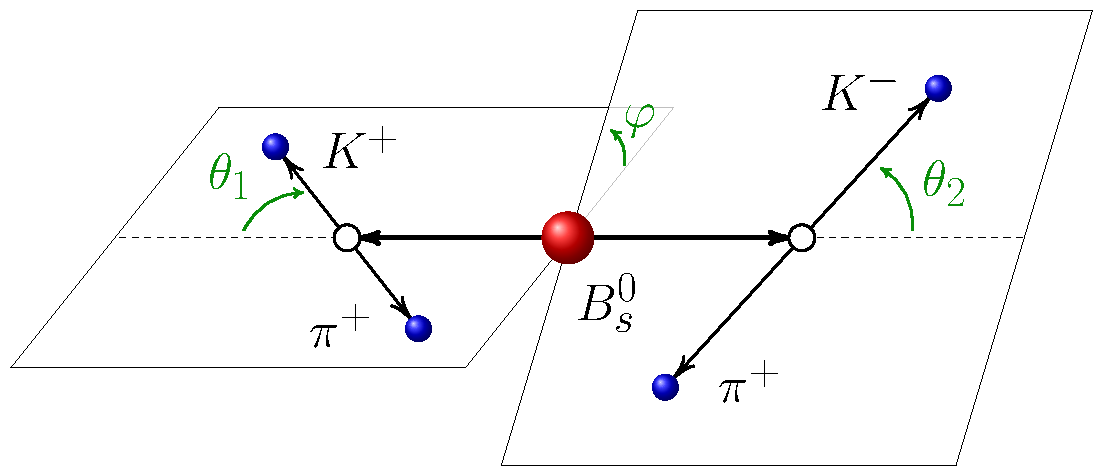
\includegraphics[width=0.7\linewidth]{diagram}
  \end{center}
  \caption{Definition of the angles $\theta_1$, $\theta_1$ and $\varphi$
   in the \decay{\Bs}{\Kstarz\Kstarzb} decay. Image by Julian Garcia Pardinas.}
  \label{fig:diagram}
\end{figure}
%%%%%%%%%%%%%%%%%%%%%%%%%%%%%%%%%%%%%%%%

%%%%%%%%%%%%%%%%%%%%%%%%%%%%%%%%%%%%%%%%%%%%%%%%%%%%%%%%%%%%%%%%%%%%%%%%%%%%%%%%%%%%%%%%%%%%%%%%%
\section{References}
\label{sec:References}

References should be made using Bib\TeX~\cite{BibTeX}. A special style
\texttt{LHCb.bst} has been created to achieve a uniform
style. Independent of the journal the paper is submitted to, the
preprint should be created using this style. Where arXiv numbers
exist, these should be added even for published articles. In the PDF
file, hyperlinks will be created to both the arXiv and the published
version, using the {\tt doi} for the latter.

Results from other experiments should be cited even if not yet published. 

\begin{enumerate}

\item Citations are marked using square brackets, and the
  corresponding references should be typeset using Bib\TeX\ and the
  official \lhcb Bib\TeX\ style. 

\item For references with four or less authors all of the authors'
  names are listed~\cite{Lee:1967iu}, otherwise the first author
  is given, followed by \etal. The \lhcb Bib\TeX\ style will
  take care of this. The limit of four names can be changed by changing the number 4 in 
  ``{\tt \#4 'max.num.names.before.forced.et.al :=}''
  in {\tt LHCb.bst}, as was done in Ref.~\cite{LHCb-PAPER-2017-038}.

\item The order of references should be sequential when reading the
  document. This is automatic when using Bib\TeX.

\item The titles of papers should in general be included. To remove
  them, change \texttt{\textbackslash
    setboolean\{articletitles\}\{false\}} to \texttt{true} at the top
  of this template.

\item Whenever possible, use references from the supplied files
\verb!main.bib!, \verb!LHCb-PAPER.bib!, \verb!LHCb-CONF.bib!, and \verb!LHCB-DP.bib!.
These are kept up-to-date by the EB. If you see a mistake, do not edit these files,
but let the EB know. This way, for every update of the paper, you save
yourself the work of updating the references. Instead, you can just copy or
check in the latest versions of the \verb!.bib! files from the repository.
{\bf Do not take these references from \texttt{inspirehep} instead} (``{\tt Aaaij:20XXxyz}''), as \texttt{inspirehep} sometimes adds mistakes, does not handle errata properly and does not use LHCb-specific macros.

\item For those references not provided by the EB, the best
  is to copy the Bib\TeX\ entry directly from
  \href{http://inspirehep.net}{inspirehep}.
    Often these need to be edited to get the 
  correct title, author names and formatting. The warning about special UTF8 characters should never be ignored. It usually signals a accentuated character in an author name.
  For authors with multiple initials, add a space between them (change \texttt{R.G.C.} to \texttt{R. G. C.}),
  otherwise only the first initial will be taken. 
  Also, make sure to eliminate unnecessary capitalisation.
  Apart from that, the title should be respected as much as possible
  (\eg do not change particle names to PDG convention nor introduce/remove factors of $c$, but do change Greek capital letters to use our slanted font.).
  Check that both the arXiv and the journal index are clickable
  and point to the right article.

%\item Even if the basic formatting of the Bib\TeX\ entry is taken from
%  \texttt{Inspire}, all the data should be cross checked against the
%  journal. Often there are minor changes to author initials or
%  titles. In case of a difference between the preprint and the
%  journal, the bibliographic information from the journal should be
%  used.

\item The \texttt{mciteplus}~\cite{mciteplus} package is used
  to enable multiple references to show up as a single item in the
  reference list. As an example \texttt{\textbackslash
    cite\{Cabibbo:1963yz,*Kobayashi:1973fv\}} where the \texttt{*}
  indicates that the reference should be merged with the previous
  one. The result of this can be seen in
  Ref.~\cite{Cabibbo:1963yz,*Kobayashi:1973fv}. Be aware that the
  \texttt{mciteplus} package should be included as the very last item
  before the \texttt{\textbackslash begin\{document\}} to work
  correctly.

\item It should be avoided to make references to public notes and
  conference reports in public documents. Exceptions can be discussed
  on a case-by-case basis with the review committee for the
  analysis. In internal reports they are of course welcome and can be
  referenced as seen in Ref.~\cite{LHCb-CONF-2012-013} using the
  \texttt{lhcbreport} category. For conference reports, omit the
  author field completely in the Bib\TeX\ record.

\item To get the typesetting and hyperlinks correct for \lhcb reports,
  the category \texttt{lhcbreport} should be used in the Bib\TeX\
  file. See Refs.~\cite{LHCb-INT-2011-047, *LHCb-ANA-2011-078,
    *CERN-THESIS-2014-057, *LHCb-PROC-2014-017, *LHCb-TALK-2014-257}
  for some examples. It can be used for \lhcb documents in the series
  \texttt{CONF}, \texttt{PAPER}, \texttt{PROC}, \texttt{THESIS},
  \texttt{LHCC}, \texttt{TDR} and internal \lhcb reports. Papers sent
  for publication, but not published yet, should be referred with
  their \texttt{arXiv} number, so the \texttt{PAPER} category should
  only be used in the rare case of a forward reference to a paper.

\item Proceedings can be used for references to items such as the
  \lhcb simulation~\cite{LHCb-PROC-2011-006}, where we do not yet have
  a published paper.

\end{enumerate}

There is a set of standard references to be used in \lhcb that are
listed in Appendix~\ref{sec:StandardReferences}.
